\scanpage{12}
\margin{\figure{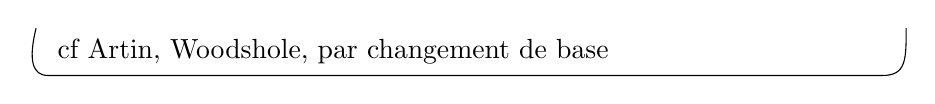
\begin{tikzpicture}\node[anchor=west] at (0,0) {cf Artin, Woodshole, par changement de base};\draw (-.15,.3) .. controls (-.25,-.1) and (-.2,-.3) .. (0,-.3)--(10.6,-.3) .. controls (10.9,-.3) and (10.9,-.1) .. (10.9,.3);\end{tikzpicture}}}

11) \uline{Supports}
\deleted{\unsure{Soient} \unsure{donc} \unsure{un} ouvert $U$ de $X$,}

\deleted{\unsure{a}} Faisceau final : $X/X$ lui-même
\[X(X')=\{e\}\]
Les sous faisceaux du faisceau final sont les ouverts de $X$.

\deleted{Support d'un $f$}
\deleted{Si $F$ est un \unsure{fai}}
La catégorie des faisceaux $F$ sur $X$ qui sur $U$ sont le faisceau final équivaut à la catégorie des faisceaux sur $Y=X-U$, par le foncteur image directe.

De $=$, faisceaux abéliens sur $X$ nuls sur $U$ $=$ faisceaux abéliens sur $Y$.

Support d'un faisceau abélien
\deleted{$\Gamma_Y(F)\subset\Gamma(F)$ \unsure{Défin.}}

Support d'une section d'un faisceau abélien
\[
\Gamma_Y(F)\subset\Gamma(F)
\]
\[
\underline\Gamma_Y(F)\subset F
\qquad
\underline\Gamma_Y(F)(X')=\Gamma_{Y'}(X',F')
\]

Foncteurs dérivés
\[
\left\{\begin{aligned}
H^i_Y(X,F)&\simeq\operatorname{Ext}^i(X;\mathbf Z_Y,F)\\
\underline H^i_Y(F)&\simeq\underline{\operatorname{Ext}}^i(\mathbf Z_Y,F)\\
&\text{'' } R^{i-1}u_*(F|U)\qquad\text{si }i\geq2
\end{aligned}\right.
\]
\margin{cf SGA 1962 ou Notes Hartshorne 1961}
\margin{si $i=0$ ou $1$, \unsure{donne} le noyau et conoyau de $F\to u_*(F)$}
\[
\text{Suite}\left\{\begin{array}{l}\text{exacte}\\\text{spectrale.....}\end{array}\right.
\]

12) \uline{Pureté}
\diagram{\begin{tikzcd}
Y \arrow[rr,phantom,"\subset"] \arrow[dr,no head,"\text{lisse}"'] && X \arrow[dl,no head,"\text{lisse}"]\\
& k &
\end{tikzcd}}
réguliers, $\operatorname{codim}_X(Y)=p$ en chaque pt de $Y$
\[
\left\{\begin{aligned}
\underline H^i_Y((\mathbf Z/n\mathbf Z)_X)&=0&&\text{si }i\neq2p\\
&\simeq\mu_n^{\otimes(-p)}&&\text{si }i=2p
\end{aligned}\right.
\]
\margin{$n$ premier aux car. résiduelles de $Y$}
\margin{Donner \unsure{définition} de la classe fondamentale \deleted{$X$ \unsure{lisse}} locale}
\mspage{11}
